%%%%%%%%%%%%%%%%%%%%%%%%%%%%%%%%%%%%%%%%%
% Structured General Purpose Assignment
% LaTeX Template
%
% This template has been downloaded from:
% http://www.latextemplates.com
%
% Original author:
% Ted Pavlic (http://www.tedpavlic.com)
%
% Note:
% The \lipsum[#] commands throughout this template generate dummy text
% to fill the template out. These commands should all be removed when 
% writing assignment content.
%
%%%%%%%%%%%%%%%%%%%%%%%%%%%%%%%%%%%%%%%%%

\documentclass{article}

\usepackage{fancyhdr} % Required for custom headers
\usepackage{lastpage} % Required to determine the last page for the footer
\usepackage{extramarks} % Required for headers and footers
\usepackage{graphicx} % Required to insert images
\usepackage[utf8]{inputenc}

% Margins
\topmargin=-0.45in
\evensidemargin=0in
\oddsidemargin=0in
\textwidth=6.5in
\textheight=9.0in
\headsep=0.25in 

\linespread{1.1} % Line spacing



\setlength\parindent{0pt} % Removes all indentation from paragraphs

%----------------------------------------------------------------------------------------
%	DOCUMENT STRUCTURE COMMANDS
%	Skip this unless you know what you're doing
%----------------------------------------------------------------------------------------

% Header and footer for when a page split occurs within a problem environment
\newcommand{\enterProblemHeader}[1]{
\nobreak\extramarks{#1}{#1 continued on next page\ldots}\nobreak
\nobreak\extramarks{#1 (continued)}{#1 continued on next page\ldots}\nobreak
}

% Header and footer for when a page split occurs between problem environments
\newcommand{\exitProblemHeader}[1]{
\nobreak\extramarks{#1 (continued)}{#1 continued on next page\ldots}\nobreak
\nobreak\extramarks{#1}{}\nobreak
}

\setcounter{secnumdepth}{0} % Removes default section numbers
\newcounter{homeworkProblemCounter} % Creates a counter to keep track of the number of problems

%----------------------------------------------------------------------------------------
%	NAME AND CLASS SECTION
%----------------------------------------------------------------------------------------

\newcommand{\lessonNumber}[1]{Lezione\ \##1} % Assignment title
\newcommand{\lessonDate}[4]{#1,\ #2\ #3\ #4} % Due date
\newcommand{\lessonCourse}[1]{#1} % Course/class
\newcommand{\lessonTime}[1]{#1} % Class/lecture time
\newcommand{\lessonTeacher}[1]{#1} % Teacher/lecturer
\newcommand{\lessonAuthor}[1]{#1} % Your name
\begin{document}
\section{Amministrazione di progetto(5)}

Si tratta di equipaggiare, organizzare e gestire l'ambiente di lavoro e produzione, attraverso regole procedure e strumenti che supportano il \textit{Way of Working}.
L'amministratore costruisce l'ambiente di lavoro e lo tiene aggiornato e funzionante. Un servizio utile deve essere anche \textbf{garantito}:

\begin{itemize}

	\item Disponibile quando serve;
	\item Ha sufficiente capacità di svolgere tutte le richieste che arrivano;
	\item Continuo;
	\item Sicuro.

\end{itemize}
Se ha queste caratteristiche agevola l'utente nel raggiungimento dei sui obbiettivi senza costi/rischi specifici.

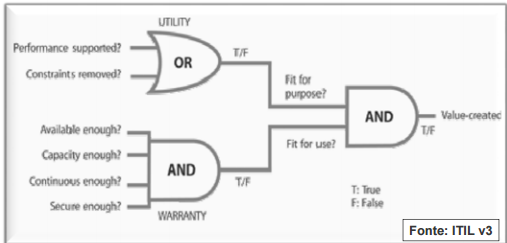
\includegraphics[width=0.75\columnwidth]{img10}\\
\textit{AND} devono essere tutte soddisfatte per proseguire \textit{OR} o una o l'altra.
\\
\\
L'amministratore arricchisce l'ambiente di servizi.\\ Tutto ruota intorno a lasciare traccia documentale di ciò che abbiamo fatto. I documenti hanno un costo e sono utili se sono \textbf{sempre disponibili} quindi devono essere:
\begin{itemize}
	\item Chiaramente identificati;
	\item Corretti nei contenuti;
	\item Verificati e approvati;
	\item Aggiornati, datati e dotati di versione.
\end{itemize}

\textbf{L'ambiente di lavoro} (\textit{strumenti a disposizione}) è fatto da regole, procedure, servizi e strumenti, deve essere:
\begin{itemize}
	\item \textbf{Completo:} ho tutto ciò che mi serve prima che mi serva;
	\item \textbf{Ordinato:} è facile trovare quello che si cerca;
	\item \textbf{Aggiornato:} il materiale vecchio non deve creare intralcio.
\end{itemize}
L'ambiente di lavoro dunque conterrà:
\begin{itemize}
	\item \textbf{Risorse HD:} strumenti di base di calcolo e di persistenza (server), la rete su cui interconnetteremo postazioni di lavoro e archivi fisici;
	\item \textbf{Risorse SW:} ambienti di sviluppo, prova, studio, con queste risorse posso costruirmi una \textit{dashboard} con la quale vedo come sto andando. Serve per avere sempre disponibile lo stato di sistema.
\end{itemize}

\textbf{Configurazione:} \fbox{\textbf{Def:} un sistema è l'unione \textbf{ordinata} di più \textbf{parti}}. E' il modo in cui tutti sanno il proprio ruolo e lo svolgono al meglio(\textbf{Best practice}. Il project manager e il responsabile controllano la configurazione, le regole per la configurazione vanno pianificate e la gestione va automatizzata.\\
Le attività sono:
\begin{itemize}
	\item Identificazione di configurazione, ogni CI (\textit{Configuration Item}) ha un'identità unica
	\item Controllo di baseline \fbox{\textbf{Def:} punto da dove non torno più indietro una volta raggiunto} (solitamente coincidono con il numero di stati di avanzamento del progetto che solitamente sono stabilite secondo:\begin{itemize}
		\item Esigenze contrattuali;
		\item Esigenze strategiche (mitigazione dei rischi);
		\item Esigenze di mercato.
	\end{itemize} è l'insieme di CI consolidato ad una specifica \textbf{milestone}
	\item Gestione delle modifiche, ogni richiesta/proposta di modifica va inoltrata in modo formale. Bisogna in oltre tenere anche traccia di queste richieste attraverso un \textit{Issue tracking};
	\item Controllo di versione, ci si appoggia su un \textbf{repository} supportato dalla tecnologia "\textit{cloud}" (es. Git), permette a ciascuno di lavorare su vecchi e nuovi CI senza il rischio di sovrascrivere, in oltre in questo modo si verifica la bontà di ogni modifica di baseline tramite la build.
\end{itemize}

Ogni singolo CI ha quindi una storia ramificata che non è necessariamente simmetrica con la versione del sistema. La storie possono essere lineari o ramificate quando ho delle varianti in cui ho più requisiti in contrasto. No solo nel codice ci devono essere le modifiche ma anche nel repository devo avere un \textit{log}.\\
\\

\textbf{Norme di Progetto} \fbox{\textbf{Def:} Linee guida per le attività di sviluppo}, sono uno strumento operativo di complemento alle procedure.\\
Obbiettivi delle norme di codifica:

\begin{itemize}
	\item \textbf{Leggibilità:} come forma di prevenzione (Verificabilità, Manutenibilità, Portabilità);
	\item \textbf{Indentazione del codice:} nomi di tipi, di variabili e funzioni devono essere espressivi e distinguere di cosa stiamo parlando. Strutturazione del codice in moduli, file, directory... Il codice va frantumato in parti piccole, che consentano di rispettare un vincolo di linee di codice per file;
	\item \textbf{Intestazione del codice:} regolazione rispetto a come uso un linguaggio. Il programmatore non può prendersi la libertà di utilizzare come vuole un linguaggio, l'\textit{header}) che deve dirmi tutto di quel modulo (cosa fa, chi l'ha fatto, copyright, copyleft, avvertenze...).

\end{itemize}

\end{document}